\newpage

\renewcommand{\thesubsection}{\textcolor{red}{\Roman{section}.\arabic{subsection}}}
\renewcommand{\thesubsubsection}{\textcolor{red}{\Roman{section}.\arabic{subsection}.\alph{subsubsection}}}

\setcounter{section}{0}
\sndEnTeteMethodoDeux


\begin{mdframed}[style=titr, leftmargin=60pt, rightmargin=60pt, innertopmargin=7pt, innerbottommargin=7pt, innerrightmargin=8pt, innerleftmargin=8pt]

\begin{center}
\large{\textbf{Fiche méthode 2 : La verrerie en chimie}}
\end{center}
\end{mdframed}

%\begin{center}
%    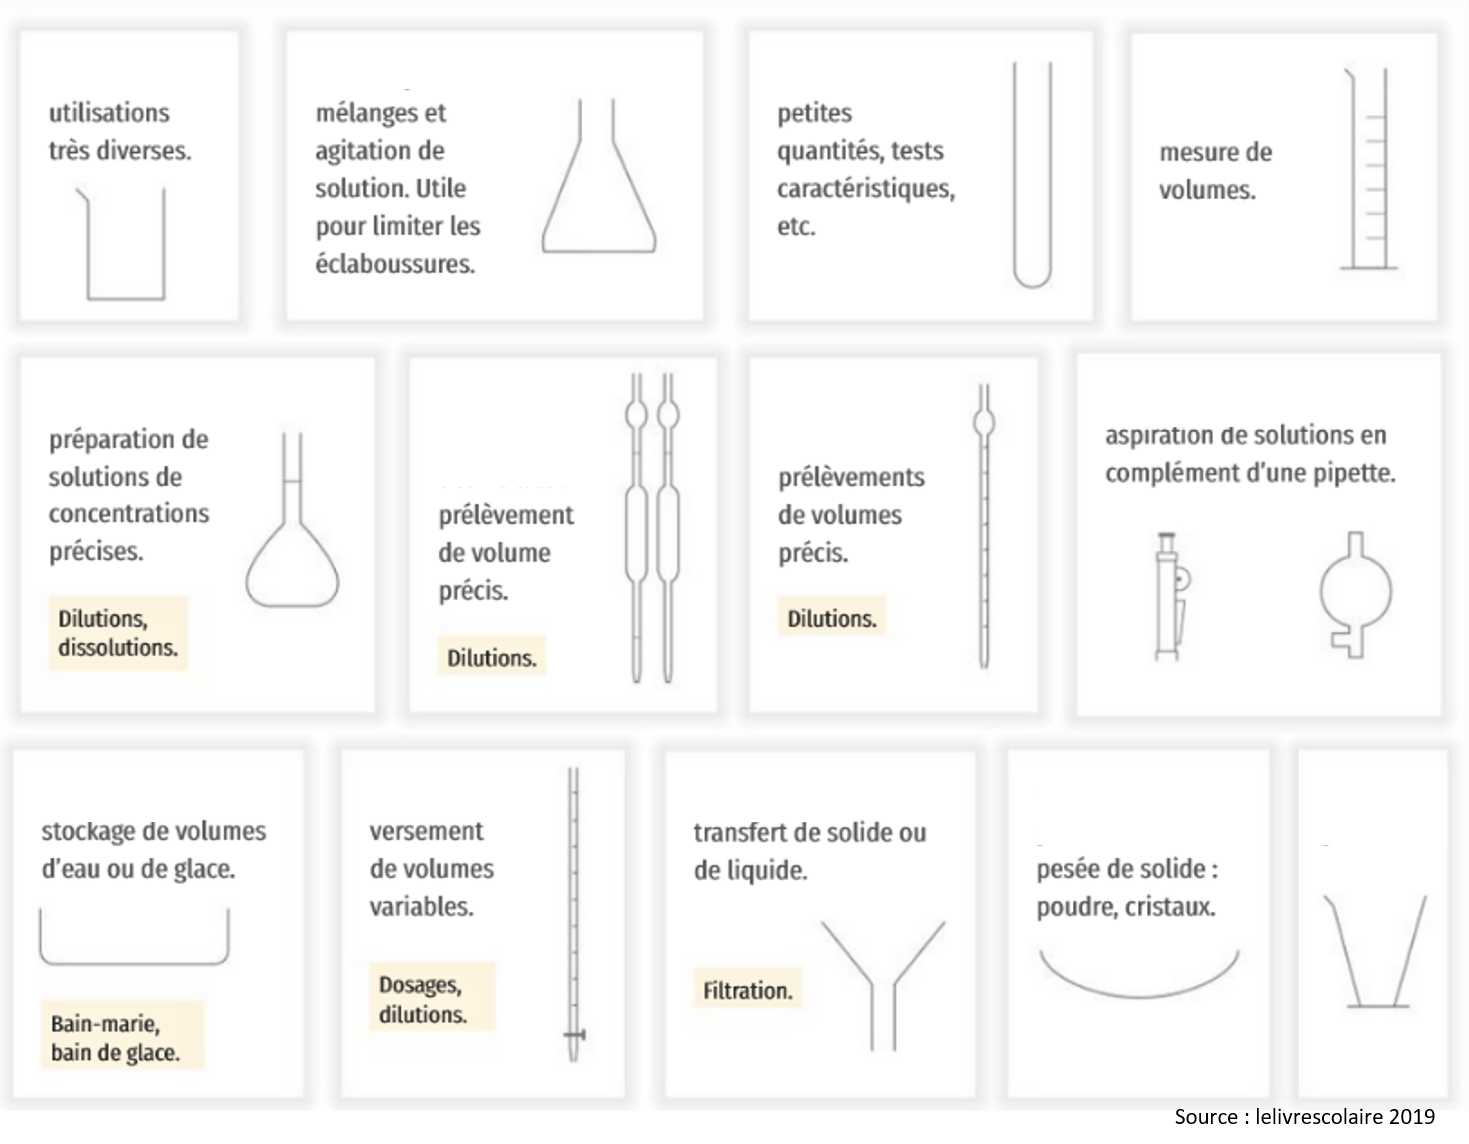
\includegraphics[scale=0.75]{Images/Methodo/Verrerie/Verrerie_acompleter.png}
%\end{center}

\begin{center}
    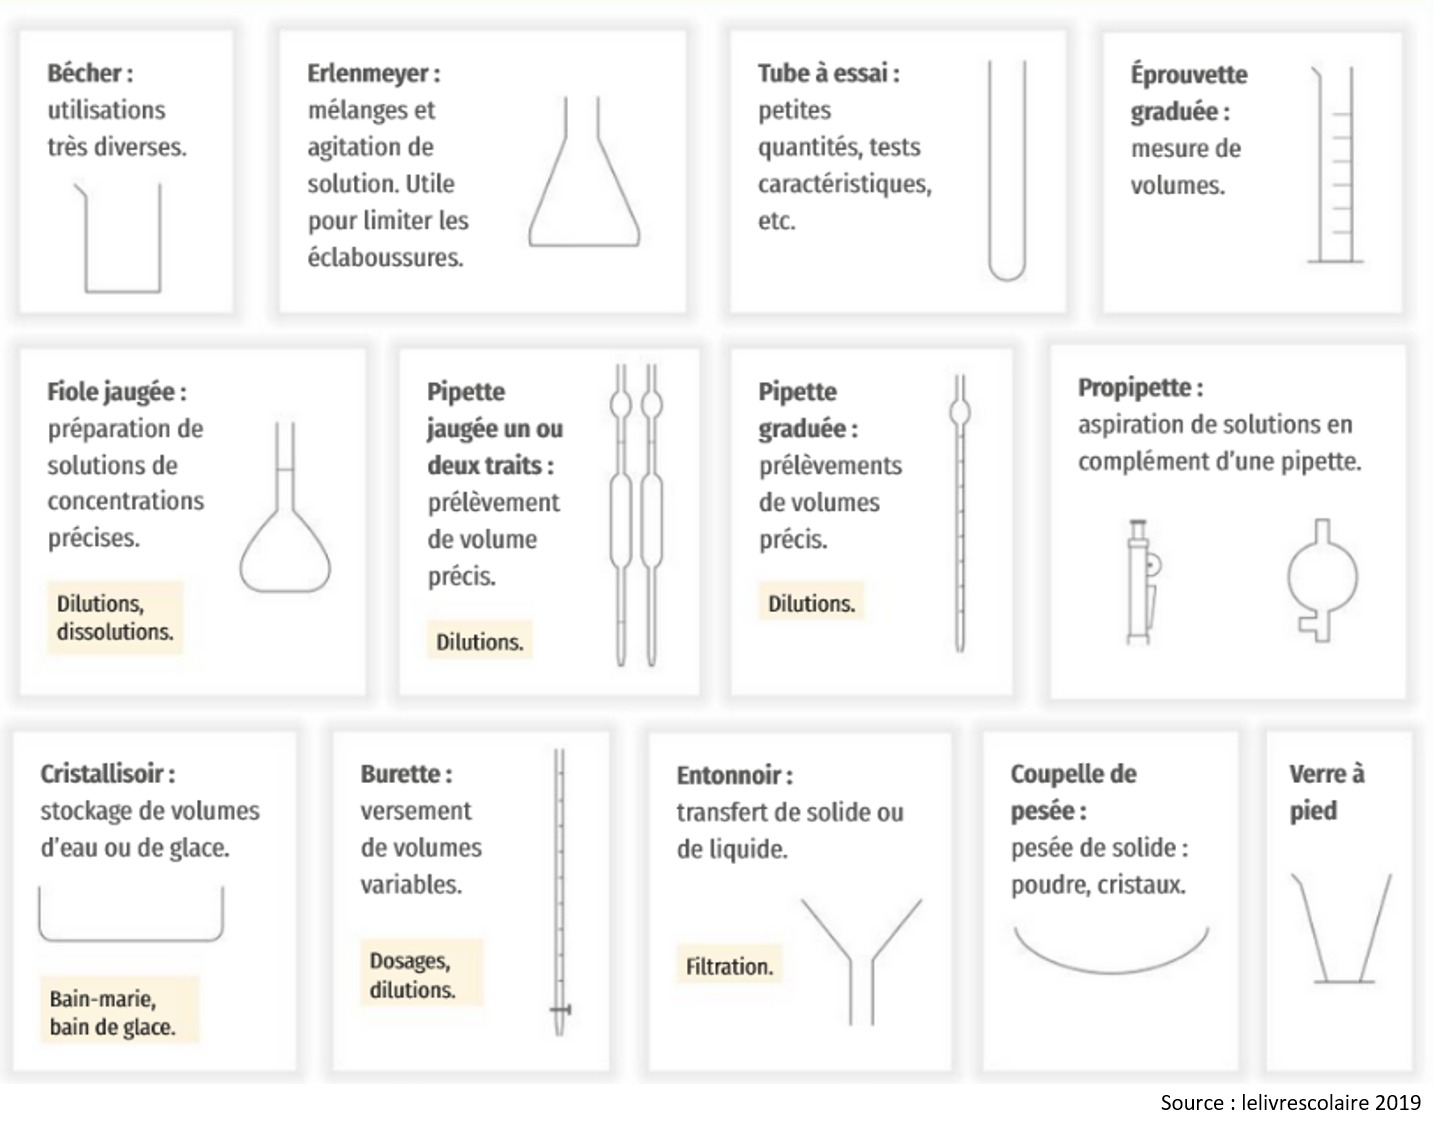
\includegraphics[scale=0.75]{Images/Methodo/Verrerie/Verrerie_completer.png}
\end{center}

